\section{Threads}

\paragraph{Processes vs. Threads}
\begin{itemize}
  \item \textbf{Traditional OS}: each process has
  \begin{itemize}
    \item own address space
    \item own set of allocated resources
    \item \emph{one} thread of execution ( = one execution state)
  \end{itemize}
  \item \textbf{Modern OS}: processes + threads of execution handled more flexibly
  \begin{itemize}
    \item \emph{processes} provide abstraction of address space and resources
    \item \emph{threads} provide abstraction of execution states of that address space
  \end{itemize}
  \item \textbf{Exceptions}:
  \begin{itemize}
    \item sometimes different threads have different address spaces
    \item \emph{Linux}: threads = regular processes with shared resources and AS regions
  \end{itemize}
\end{itemize}

\paragraph{Threads --- why?}
\begin{itemize}
  \item many programs do multiple things at once (e.g. web server)
  \begin{itemize}
    \item[$ \leadsto $] writing program as many sequential threads may be easier than with blocking operations
  \end{itemize}
  \item \textbf{Processes}: rarely share data (if, then explicitly)
  \item \textbf{Threads}: closely related, share data
\end{itemize}
\begin{figure}[h]\centering\label{ProcessesThreads}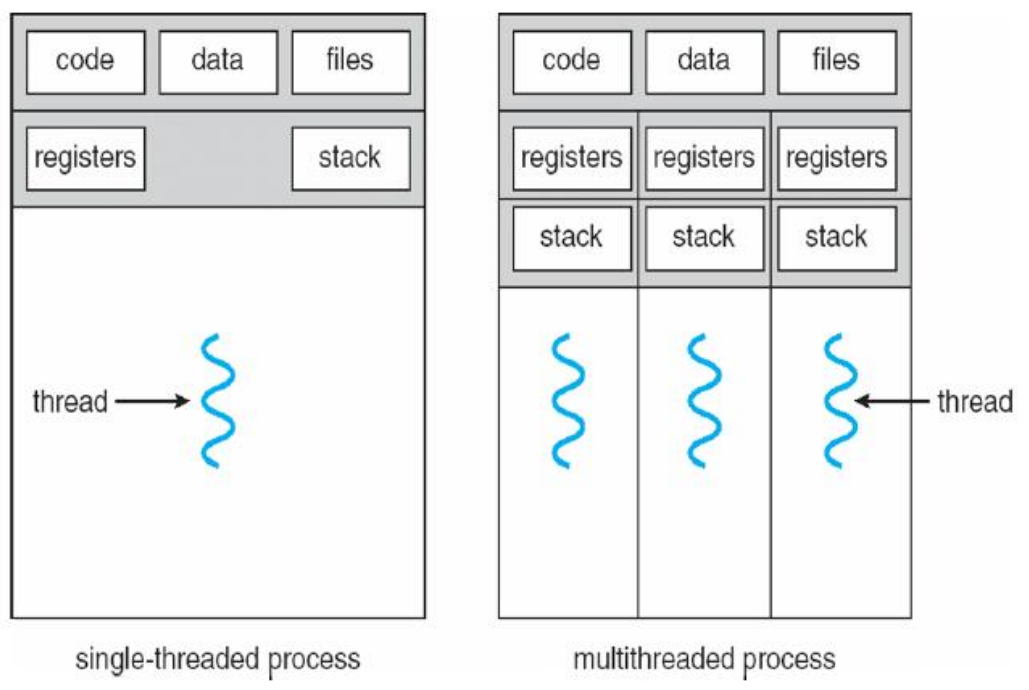
\includegraphics[width=0.33\textwidth]{ProcessesThreads}\end{figure}

\paragraph{Threads --- POSIX}
\begin{itemize}
  \item \code{PThread}: base object with
  \begin{itemize}
    \item \emph{identifier} (thread ID, TID)
    \item \emph{register set} (including IP and SP)
    \item \emph{stack area} to hold execution state
  \end{itemize}
  \item \code{Pthread_create}: create new thread
  \begin{itemize}
    \item Pass: \emph{pointer} to \code{pthread_t} (will hold TID after successful call)
    \item Pass: \emph{attributes}, \emph{start function}, \emph{arguments}
    \item Returns: \code{0} on success, error value else
  \end{itemize}
  \item \code{Pthread_exit}: terminate calling thread
  \begin{itemize}
    \item Pass: exit code (casted to void pointer)
    \item Free's resources (e.g. stack)
  \end{itemize}
  \item \code{Pthread_join}: wait for specified thread to exit
  \begin{itemize}
    \item Pass: \code{ptread_t} to wait for (or \code{-1} for any thread)
    \item Pass: pointer to pointer for exit code
    \item Returns: \code{0} on success, error value else
  \end{itemize}
  \item \code{Pthread_yield}: release CPU to let another thread run
\end{itemize}

\paragraph{Threads --- Problems}
\begin{itemize}
  \item \textbf{Processes vs. Threads}:
  \begin{itemize}
    \item \emph{Processes}: only share resources explicitly
    \item \emph{Threads}: more shared state \( \to \) more can go wrong
  \end{itemize}
  \item \textbf{Challenges}: programmer needs to take care of
  \begin{itemize}
    \item \emph{activities}: dividing, ordering, balancing
    \item \emph{data}: dividing
    \item \emph{shared data}: access synchronizing
  \end{itemize}
\end{itemize}

\paragraph{PCB vs. TCP}
\begin{itemize}
  \item \textbf{PCB} (\emph{process control block}): information needed to implement processes
  \begin{itemize}
    \item always known to OS
  \end{itemize}
  \item \textbf{TCB} (\emph{thread control block}): per thread data
  \begin{itemize}
    \item OS knowledge depends on \emph{thread model}
  \end{itemize}
\end{itemize}
\begin{figure}[H]\centering\label{PCBTCB}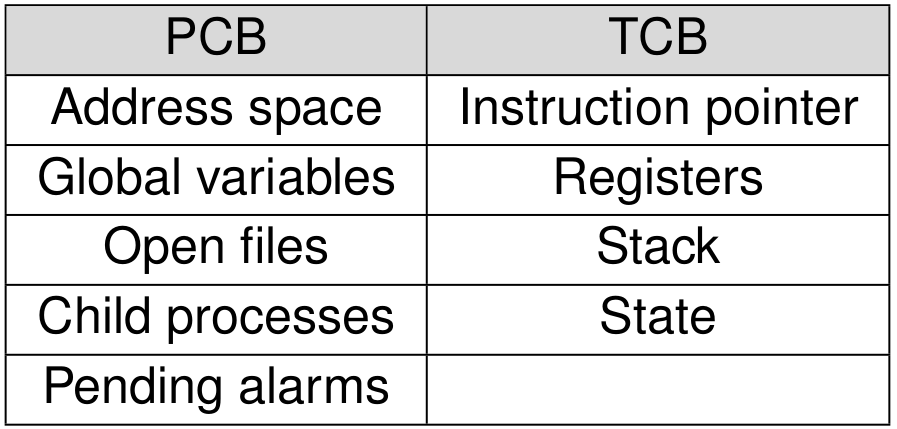
\includegraphics[width=0.2\textwidth]{PCBTCB}\end{figure}

\paragraph{Thread models}
\begin{itemize}
  \item \textbf{Kernel Thread}: known to OS kernel
  \item \textbf{User Thread}: known to process
  \item \textbf{N:1-Model}: kernel only knows one of possibly multiple threads
  \begin{itemize}
    \item N:1 user threads = \emph{user level threads} (ULT)
  \end{itemize}
  \item \textbf{1:1-Model}: each user thread maps to one kernel thread
  \begin{itemize}
    \item 1:1 user threads = \emph{kernel level threads} (KLT)
  \end{itemize}
  \item \textbf{M:N-Model} (hybrid model): flexible mapping of user threads to less kernel threads 
\end{itemize}

\paragraph{Thread models --- N:1}
\begin{itemize}
  \item Kernel only manages process \( \to \) multiple threads unknown to kernel 
  \item Threads managed in user-space library (e.g. GNU Portable Threads)
  \item \textbf{Pro}:
  \begin{itemize}
    \item[+] faster thread management operations (up to 100 times)
    \item[+] flexible scheduling policy
    \item[+] few system resources
    \item[+] usable even if OS doesn't support threads
  \end{itemize}
  \item \textbf{Con}:
  \begin{itemize}
    \item[-] no parallel execution
    \item[-] whole process blocks if one user thread blocks
    \item[-] reimplementing OS parts (e.g. scheduler)
  \end{itemize}
  \item \textbf{Stack}:
  \begin{itemize}
    \item main stack known to OS used by thread library
    \item own execution state (= stack) dynamically allocated by user thread library for each thread
    \item possibly own stack for each exception handler
  \end{itemize}
  \item \textbf{Heap}:
  \begin{itemize}
    \item concurrent heap use possible
    \item \emph{Attention}: not all heaps are reentrant
  \end{itemize}
  \item \textbf{Data}: divided into BSS, data and read-only data here as well
\end{itemize}
\begin{figure}[h]\centering\label{ULTAddressSpace}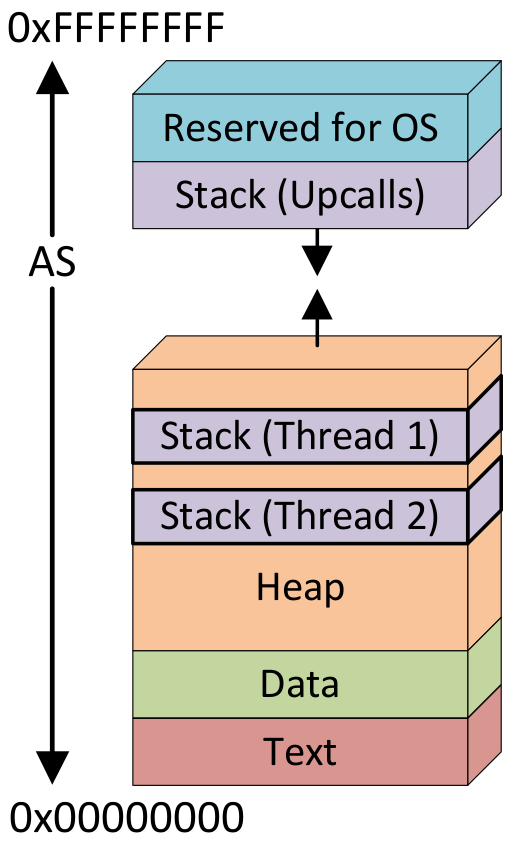
\includegraphics[width=0.15\textwidth]{ULTAddressSpace}\end{figure}

\paragraph{Thread models --- 1:1}
\begin{itemize}
  \item kernel knows + manages every thread
  \item \textbf{Pros}:
  \begin{itemize}
    \item[+] real parallelism possible
    \item[+] threads block individually
  \end{itemize}
  \item \textbf{Cons}:
  \begin{itemize}
    \item[-] OS manages every thread in system (TCB, stacks,\dots)
    \item[-] Syscalls needed for thread management
    \item[-] scheduling fixed in OS
  \end{itemize}
  \item \textbf{Stack}:
  \begin{itemize}
    \item own execution state (= stack) for every thread
    \item possibly own stack for (each) exception handler
  \end{itemize}
  \item \textbf{Heap}:
  \begin{itemize}
    \item parallel heap use possible
    \item \emph{Attention}: not all heaps are thread-safe
    \item if thread-safe: not all heap implementations perform well with many threads
  \end{itemize}
  \item \textbf{Data}: divided into BSS, data and read-only data here as well
\end{itemize}
\begin{figure}[h]\centering\label{KLTAddressSpace}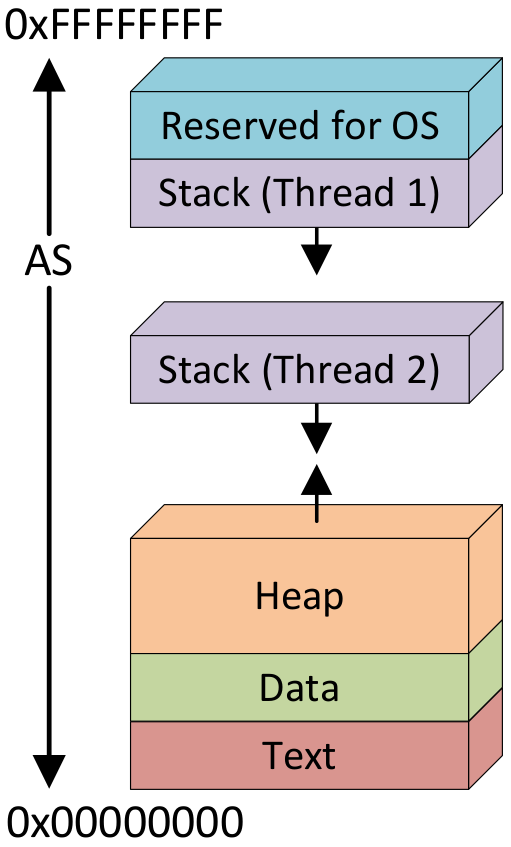
\includegraphics[width=0.15\textwidth]{KLTAddressSpace}\end{figure}

\paragraph{Thread models --- M:N}
\begin{itemize}
  \item \textbf{Principle}: \( M \) ULTs are maps to (at most) \( N \) KLT
  \begin{itemize}
    \item \emph{Goal}: pros of ULT and KLT --- non-blocking with quick management
    \item create sufficient number of KLTs and flexibly allocate ULTs to them
    \item \emph{Idea}: if ULT blocks ULTs can be switched in userspace
  \end{itemize}
  \item \textbf{Pros}:
  \begin{itemize}
    \item[+] flexible scheduling policy
    \item[+] efficient execution
  \end{itemize}
  \item \textbf{Cons}:
  \begin{itemize}
    \item[-] hard to debug
    \item[-] hard to implement (e.g. blocking, number of KLTs,\dots)
  \end{itemize}
  \item \textbf{Implementation --- Up-calls}:
  \begin{itemize}
    \item kernel notices that thread will block \( \to \) sends signal to process
    \item up-call notifies process of thread id and event that happened
    \item exception handler of process schedules a different process thread
    \item kernel later informs process that blocking event finished via other up-call
  \end{itemize}
\end{itemize}

\begin{summary}
  \begin{itemize}
    \item programs often do closely related things at once
    \begin{itemize}
      \item mapped to thread abstraction: multiple threads of execution operate in same process
    \end{itemize}
    \item differentiation between process information (PCB) and thread information (TCB)
    \item \textbf{thread models}:
    \begin{itemize}
      \item $ N:1 $: threads fully managed in user-space
      \item $ 1:1 $: threads fully managed by kernel
      \item $ M:N $: threads are flexibly managed either in user-space or kernel
    \end{itemize}
    \item multi-threaded programs operate on same data concurrently or even parallel:
    \begin{itemize}
      \item \emph{synchronization}: accessing such data must be synchronized
      \item[$ \to $] makes writing such programs challenging
    \end{itemize}
  \end{itemize}
\end{summary}